\documentclass[11pt,letter]{report}
\usepackage[margin=1in]{geometry}
\usepackage{asymptote}
\usepackage{wrapfig}
\usepackage{gensymb}
\usepackage{amsmath}
\usepackage{tabu}

\begin{document}
\chapter*{Motion in One Dimension}

\textbf{Kinematics} Description of motion

\section*{Displacement, Velocity, and Speed}

An object moving from intial position $x_{i}$ to final position $x_{f}$ has \textbf{displacement} $$\Delta{x}=x_{f}-x_{i}.$$

\noindent
The \textbf{average velocity} of the object is the ratio of the displacement to the time it takes for the displacement $\Delta{t}=t_{f}-t_{i}$,
$$v_{av}=\frac{\Delta{x}}{\Delta{t}}.$$

\noindent
The \textbf{average speed} of the object is the ratio of the distance traveled to the time it takes, $$\bar{v}=\frac{\Delta{s}}{\Delta{t}}.$$

\noindent
The average velocity and the average speed of an object are very different.

\noindent
\textit{Geometric Interpretation}: The average velocity is the slope of the straight line connecting the points $\left(t_{1}, x_{1}\right)$ and $\left(t_{2}, x_{2}\right)$ in the $x$-versus-$t$ plot.

\noindent
\textbf{Instantaneous velocity} is defined as $$v\left(t\right)=\lim_{\Delta{t} \to 0} \frac{\Delta{x}}{\Delta{t}}.$$

\noindent
The \textbf{instantaneous speed} is the magnitude of the instantaneous velocity.

\section*{Acceleration}

The rate of change of the instantaneous velocity with respect to time.

The \textbf{average acceleration} of an object is the ratio of the \textit{change} in velocity to the time it takes for the change $\Delta{t}=t_{f}-t_{i}$, $$a_{av}=\frac{\Delta{v}}{\Delta{t}}.$$

The \textbf{instantaneous acceleration} is the slope of the line tangent to the $v$-versus-$t$ curve. $$a=\lim_{\Delta{t} \to 0} \frac{\Delta{v}}{\Delta{t}}.$$

\subsection*{Motion with Constant Acceleration}

The motion of a particle that has constant acceleration is common in nature. When air resistance is negligeble, the free fall of an object near Earth's surface has acceleration $g=9.81 m/s^{2}$, which Galileo was the first to conclude.

\noindent
We can use the ``Big Five'' under constant acceleration:
$$v=v_{0}+at$$
$$\Delta{x}=v_{0}t+\frac{1}{2}at^{2}$$
$$v^{2}-v^{2}_{0}=2a\Delta{x}$$
$$\Delta{x}=\frac{1}{2}\left(v_{0}+v\right)t$$
$$\Delta{x}=vt-\frac{1}{2}at^{2}$$

\chapter*{Vectors and Two-Dimensional Motion}

\section*{General Properties of Vectors}

A \textbf{vector quantity} has both a magnitude and a direction.\\A \textbf{scalar quantity} has magnitude, but no direction.

\hspace{1mm}

\noindent
\textit{Equality} $\vec{A}\ =\ \vec{B}$ if $A = B$ and their directions are the same.

\hspace{1mm}

\noindent
\textit{Addition} Vectors can be added both geometrically and algebraically.

\underline{Geometrically} \textsl{Head-to-tail} and \textsl{parallelogram} methods can be used.

Thus, the \textbf{resultant vector} $\vec{R}\ =\ \vec{A} + \vec{B}$ is the sum of two or more vectors.

\hspace{1mm}

\noindent
\textit{Negative} The negative of a vector has the same magintude but opposite direction.

\hspace{1mm}

\noindent
\textit{Subtraction} $\vec{A} + \vec{B}\ =\ \vec{A} + \left(-\vec{B}\right)$.

\hspace{1mm}

\noindent
\textit{Multiplication by a Scalar} $s \vec{A}$ has magnitude $sA$ and has the same direction as $\vec{A}$ if $s$ if positive and opposite direction if $s$ is negative.

\begin{wrapfigure}{r}{0.3\textwidth}
\begin{center}
\vspace{-20pt}
\begin{asy}
import graph;
xaxis("$x$", xmin=-0.5);
yaxis("$y$");
import olympiad;
	defaultpen(1.0);
	size(5cm);
	draw((0,0)--(2,1),EndArrow);
	markscalefactor=0.05;
	draw(anglemark((2,0),(0,0),(2,1)));
	draw((2,0)--(2,1),dashed);
	draw((0,1)--(2,1),dashed);
	label("$A_x = A \cos{\theta}$",(0,0)--(2,0),S);
	label("$A_y = A \sin{\theta}$",(0,0)--(0,1),W);
	dot((2.2,1.2),invisible);
\end{asy}
\vspace{-20pt}
\end{center}
\end{wrapfigure}

\hspace{1mm}

\noindent
\textit{Components} The component of $\vec{A}$ in the direction of a directed line $S$ is $A_S = A\cos{\theta}$, where $\theta$ is the angle between $S$ and $\vec{A}$.\\A vector can be specified by its rectangular components along the $x$- and $y$-axes $$A_x = A\cos{\theta},$$ $$A_y = A\sin{\theta}.$$\\It can also be specified by its magnitude and direction through the Pythagorean theorem and the definition of tangent $$A=\sqrt{A_x^2 + A_y^2},$$ $$\tan{\theta} = \frac{A_y}{A_x}.$$\\We can hence define \underline{algebraic} addition of vectors such that $$\vec{A}\ =\ \vec{A} + \vec{B}\ \Longleftrightarrow C_x = A_x + B_x \textrm{ and } C_y = A_y + B_y.$$

\section*{Position, Velocity, and Acceleration}

The \textbf{position vector} of a particle at a point $\left(x, y\right)$ is a vector from the origin to the point $$\vec{r} = x\hat{i} + y\hat{j}.$$

\noindent
The \textbf{displacement} is the change in position $$\Delta{\vec{r}} = \vec{r}_2 - \vec{r}_1.$$

\noindent
The \textbf{average velocity} in the time interval $\Delta{t} = t_2 - t_1$ $$\vec{v}_{av} = \frac{\Delta{\vec{r}}}{\Delta{t}}.$$

\noindent
The \textbf{instantaneous velocity} $$\vec{v} = \lim_{\Delta{t} \to 0} \frac{\Delta{\vec{r}}}{\Delta{t}}.$$

\noindent
The \textbf{average acceleration} in the time interval $\Delta{t} = t_2 - t_1$ $$\vec{a}_{av} = \frac{\Delta{\vec{v}}}{\Delta{t}}.$$

\noindent
The \textbf{instantaneous acceleration} $$\vec{a} = \lim_{\Delta{t} \to 0} \frac{\Delta{\vec{v}}}{\Delta{t}}.$$

\section*{Relative Velocity}

Measurements of velocity depend on the reference frame of the observer. A reference frame is just a coordinate system.

\noindent
Consider a particle of velocity $\vec{v}_{pA}$ relative to reference frame A, which has velocity $\vec{v}_{AB}$ relative to frame B, the velocity of the particle relative to frame B is then $$\vec{v}_{pB} = \vec{v}_{pA} + \vec{v}_{AB}.$$\\However, this relative-velocity realtion is only true when the velocities are small compared to the speed of light.
\section*{Projectile Motion}

Consider an object projected with an initial velocity $\vec{v}_0$ at angle angle $\theta_0$ with the horizontal surface. The components of the velocity are $$v_{0x} = v_0 \cos{\theta_0},$$ $$v_{0y} = v_0 \sin{\theta_0}.$$

\noindent
In the absense of air resistance, the motion of the projectile is the superposition of a constant-velocity motion in the $x$-direction and a constant-acceleration in the $y$-direction. $$a_x = 0,$$ $$a_y = -g.$$

\noindent
Thus, the kinematics of one-dimensional motion can be applied $$\Delta{x} = v_{0x} t,$$ $$v_y = v_{0y} - gt,$$ $$\Delta{y} = v_{0y} t - \frac{1}{2} gt^2,$$ $$v_y^2 - v_{0y}^2 = -2g \Delta{y}.$$

We can also show that the path of the projectile is a parabola $$y = x\tan{\theta_0} - \frac{1}{2} \frac{g}{v_0^2 \cos{2\theta_0}}.$$

\chapter*{The Laws of Motion}


\section{Newton's Laws}
A \textbf{force} is simply a push or a pull on some object.\\A force has both magnitude and direction, so it is a vector quantity.

\subsection{Newton's First Law}
\textit{Principle of inertia}: if an object is left alone, is not perturbed, it continues to move with a constant velocity in a straight line if it was originally moving, or it continues to stand still if it was just standing still.
\\\textbf{Inertia} The tendency of an object to continue in its original state of motion.

\hspace{1mm}

\noindent
\textbf{Mass} A measure of inertia, or the object's resistance to changes in its motion due to a force.

\hspace{1mm}

\noindent
Newton formalized Galileo's principle of inertia into \textbf{Newton's first law of motion}:\\\emph{An object moves with a constant velocity unless acted upon by a nonzero net force.}

\subsection{Newton's Second Law}
Newton's second law provides a specific way of determining how the velocity of an object changes under different influences called forces.
\emph{The acceleration of an object is directly proportional to the net force acting on it and inversely proportional to its mass.}
$$\vec{a} = \frac{\sum \vec{F}}{m} \mathrm{, or } \sum{\vec{F}} = \vec{F}_\mathrm{net} = m \vec{a}$$
\\When $a = 0$, we have the condition of \textbf{equilibrium}.

\hspace{1mm}

\noindent
\underline{Newton's second law is applicable on every object.}

\subsection{Unit of Force}
Newton's first and second laws allow us to define force more precisely.

\hspace{1mm}

\noindent
A \textbf{force} is an external influence on an object that causes it to accelerate relative to an inertial reference frame. The direction of the force is that of the acceleration it causes and the magnitude is the product of the mass of the object and the magnitude of the acceleration.
%intrinsic prop

\hspace{1mm}

\noindent
The SI unit of force is the newton, or N. 1 N = 1 kg m/s$^2$. In the U.S. customary system, the unit of force is the pound. 1 N = 0.225 lb. The units of mass and acceleration in the U.S. customary system are the slug and ft/s$^2$.

\subsection{Newton's Third Law}
\emph{Forces always occur in equal and opposite pairs. If object A exerts a force $\vec{F}_{A, B}$ on object B, an equal but opposite force $\vec{F}_{B, A}$ is exerted by object B on object A.} $$\vec{F}_{A, B} = -\vec{F}_{B, A}$$
The pair of forces are parts of an interaction between two objects. One force is called action and the other reaction.
\\It is important to note that action and reaction forces act on different objects.

\section{Forces in Nature}
Forces that result from the physical contact between two objects are called \textbf{contact forces}.
\\Forces that do not involve any direct physical contact and act at a distance are called \textbf{field forces}.

\subsection{Weight}The force due to gravity.
\\When air resistance is neglected, all falling objects near Earth's surface have the same acceleration (by experiment): $$g=9.81 \mathrm{ m/s} ^2 \approx 10 \mathrm{ m/s} ^2$$
The force causing this acceleration is the gravitational force on the object, called weight. If the weight is the only force acting on the object, the object is said to be in \textbf{free-fall}.

\begin{wrapfigure}{r}{0.2\textwidth}
\begin{center}
\begin{asy}
size(4cm);
draw((0,0)--(100,0));
draw((10,0)--(10,80));
draw((10,80)--(90,80));
draw((90,80)--(90,0));
dot((50,40));
draw((50,40)--(50,-10),EndArrow);
label("$m \vec{g}$",(50,40)--(50,-10),E);
dot((50,-70));
draw((50,-70)--(50,-20),EndArrow);
label("$m \vec{g'}$",(50,-70)--(50,-20),E);
draw((20,75)--(20,0),EndArrow);
label("$\vec{F}_{n}^{'}$",(20,60),E);
draw((20,-75)--(20,0),EndArrow);
label("$\vec{F}_{n}$",(20,-75)--(20,0),W);
\end{asy}
\end{center}
\end{wrapfigure}

\subsection{Contact Forces}
\begin{itemize}
	\item \textbf{Normal Force} $F_n$ Push or compression reaction force.
	\item \textbf{Tension} $T$ Force from a string or a rope when taut.
	\item \textbf{Spring Force} $F_x = -k \Delta{x}$ Force from the compression or stretching of a spring.
	\item \textbf{Friction} $f$ Parallel resistive force between two surfaces.
	\item \textbf{Drag Force} $f = b v^n$ Resistive drag force through a fluid.
\end{itemize}

\subsection{Friction} Surfaces in contact can also exert forces on each other that are parrallel to the contacting surfaces.

\hspace{1mm}

\noindent
\textbf{Static Friction} The resistive force that opposes the attempted motion of an object past another object with which it is in contact. $$f_s \leq \mu_s F_n = f_{s,max}$$ $\mu_s$ is the coefficient of static friction. It depends on the nature of the surface in contact.


\hspace{1mm}

\noindent
If you exert a horizontal force smaller than $f_{s,max}$ on a box, the frictional force will just balance this horizontal force.

\hspace{1mm}

\begin{wrapfigure}{r}{0.4\textwidth}
\begin{center}
\vspace{-20pt}
\begin{asy}
import graph;
xaxis("$F_{app}$", xmin=0);
yaxis("$f$", ymin=0);
labelx("Applied force",(45,0));
axes(ylabel="Frictional force\ \ \ \ \ ");
size(6cm);
draw((0,0)--(50,50));
draw((50,50)--(55,40));
draw((55,40)--(100,40));
draw((30,10)--(10,10),EndArrow);
label("$f_{s} = F_{app}$",(30,10),E);
draw((50,70)--(50,50),EndArrow);
label("$f_{s, max} = \mu_{s} F_{n}$",(50,70),N);
draw((75,30)--(75,40),EndArrow);
label("$f_{k} = \mu_{k} F_{n}$",(75,30),S);
\end{asy}
\end{center}
\end{wrapfigure}

\noindent
\textbf{Kinetic Friction} The resistive force that opposes the motion of an object past another object with which it is in contact. It is between the surfaces of the two objects.
\\The motion has started.
\\Data show $$f_k = \mu_k F_n$$ $\mu_k$ is the coefficient of kinetic friction. It depends on the nature of the surface in contact.
\\It does not depend on velocity, so it is constant once the motion starts.
\\Experimentally, $\mu_k < \mu_s$.
\chapter*{Energy}

\section{Work}
The \textbf{work} done by a constant force $\vec{F}$ that moves an object a displacement $\Delta{x}$ is defined as $$W \equiv F \Delta{x} \cos{\theta}.$$ So $W = \vec{F} \cdot \Delta{\vec{x}}$.

\noindent
Work is a scalar. The SI unit of work is the \textit{joule} (J), $1 \mathrm{\ J} = 1 \mathrm{\ N} \cdot \mathrm{m} = 1 \mathrm{\ kg} \cdot \mathrm{m}^2 / \mathrm{s}^2$.

\smallskip

\noindent
A \textbf{particle} is any object where all of its parts undergo equal $\Delta{x}$ over any $\Delta{t}$.
\\The total work done on a particle is the same as the work done by the net force on the particle, so the work done is the area under the $F_x$-versus-$x$ curve: $$W = \sum{\vec{F_i}} \cdot \Delta{\vec{x}} = \vec{F}_\mathrm{net} \cdot \Delta{\vec{x}}.$$

\section{Kinetic Energy}
Under a constant \textit{net} force $F_\mathrm{net}$ acting along a straight line on a particle of mass $m$, which is displaced by $\Delta{x}$ along the straight line, the work done on the particle is $$W = F_\mathrm{net} \Delta{x}.$$
Applying Netwon's second law $F_\mathrm{net} = ma$ and the kinematic relation $v^2 - v_0^2 = 2a \Delta{x}$, we have $$W = F_\mathrm{net} \Delta{x} = ma \Delta{x} = \frac{1}{2} mv^2 - \frac{1}{2} mv_0^2.$$
The quantity $\frac{1}{2} mv^2$ is defined as the \textbf{kinetic energy} of the particle $$K \equiv \frac{1}{2} mv^2.$$
\\Kinetic energy is a scalar. The SI unit of kinetic energy is the same as work: $\mathrm{kg} \cdot \mathrm{m}^2 / \mathrm{s}^2$ or J.
\\Kinetic energy depends on the mass and speed of the particle but not the direction of motion.

\smallskip

\noindent
$W = \Delta{K}$. This is true even when the force is varying. This is known as the \textbf{work-energy theorem}.

\section{Potential Energy}
The \textbf{potential energy} of a system is the energy associated with the configuration of the system. Often the work done by external forces on a system may result in an increase in the potential energy of the system.

\smallskip

\noindent
\textit{Gravitational Potential Energy} The gravitational force between an object of mass $m$ and the Earth is $\vec{F} = -mg\,\hat{j}$, where $h$, $h_0 \ll r_E$, so the work done by gravity is $$W_g = \vec{F} \cdot \Delta{x} = -mg\,\hat{j} \cdot \Delta{\vec{x}} = -mg \Delta{h} = -mg \left(h - h_0\right).$$
When the object is near the surface of the Earth, the gravitational potential energy $$U_g \equiv mgh.$$
Thus, the work done by gravity is at the expense of the gravitational potential energy: $$W_g \equiv -\Delta{U_g}.$$
\textit{Potential Energy of a Spring} The work done by the spring force, $F = -kx$, is given as $$W_s = -\frac{1}{2} \left(kx_1 + kx_2\right)\left(x_2 - x_1\right) = -\left(\frac{1}{2} kx_2^2 - \frac{1}{2} kx_1^2\right).$$
When the spring potential energy is zero at $x = 0$, the spring potential energy can be defined as $$U_s \equiv \frac{1}{2} kx^2.$$
The work done by the spring force is then at the expense of the spring potential energy $$W_s = -\Delta{U_s}.$$

\subsection{Conservative Force and Potential-Energy Function}

A force is conservative if on a particle $W_\mathrm{net} = 0$ around \textit{any} closed path.
\\We can use this property to define a \textbf{potential-energy function} $U$ such that the force is the negative of the slope of the potential-energy $U$-versus-$x$ curve: $$W = \sum_i \vec{F} \cdot \Delta{\vec{x}_i} = -\Delta{U}.$$
\textbf{Non-conservative forces} are forces that are not conservative.

\section{Conservation of Mechanical Energy}
A \textbf{system} is a collection of particles. All forces are either \textbf{external} or \textbf{internal}. The change in $E_\mathrm{net}$ of a system is done through work and heat. Since $K = \sum{K_i}$, we obtain by the work-energy theorem $$W_\mathrm{net} = \sum{\Delta{K_i}} = \Delta{K} = W_\mathrm{ext} + W_\mathrm{nc} + W_\mathrm{c}.$$
The work done by all internal conservative forces can be recast as the change in the total potential energy of the system: $$W_\mathrm{c} = -\Delta{U}.$$
The sum $E_\mathrm{mech} = K + U$ is known as the total mechanical energy of the system, $$W_\mathrm{ext} + W_\mathrm{nc} = \Delta{K} + \Delta{U} = \Delta{\left(K + U\right)} = \Delta{E_\mathrm{mech}}.$$
When $W_\mathrm{ext} = 0$ and $W_\mathrm{nc} = 0$, we get the \textbf{conservation of mechanical energy}: $$K_f + U_f = K_i + U_i.$$

\section{Conservation of Energy}
For an isolated system, we have $W_\mathrm{ext} = 0$ and we may account of $W_\mathrm{nc}$ by changes in forms of energy other than mechanical energy. \textbf{The law of energy conservation:} $$E = E_\mathrm{mech} + E_\mathrm{therm} + E_\mathrm{chem} + E_\mathrm{other}.$$
Work and heat are the ways to transfer energy in or out of a system. When $\Delta{Q} = 0$, we have: $$W_\mathrm{ext} = \Delta{E} = \Delta{E_\mathrm{mech}} + \Delta{E_\mathrm{therm}} + \Delta{E_\mathrm{chem}} + \Delta{E_\mathrm{other}}.$$

\section{Power}
Power is the rate at which energy is transferred. The average \textbf{power} supplied by a force $\vec{F}$ is the rate at which the force does work: $$\bar{P} = \frac{\Delta{W}}{\Delta{t}} = \vec{F} \cdot \frac{\Delta{\vec{x}}}{\Delta{t}} = \vec{F} \cdot \vec{v}_{av},$$ $$P = \lim_{\Delta{t} \to 0} \vec{F} \cdot \vec{v}.$$
The SI unit of power is J/s, also called the \textbf{watt}. $1 \mathrm{\ W} = 1 \mathrm{\ J} / \mathrm{s} = 1 \mathrm{\ kg} \cdot \mathrm{m}^2 / \mathrm{s}^3$.

\chapter*{Momentum and Collisions}

\section{Momentum and Impulse}
The product of mass and velocity of an object is defined as the \textbf{momentum} of the object $$\vec{p} = m \vec{v}.$$
Momentum is a vector quantity. Its SI unit is $\mathrm{kg} \cdot \mathrm{m}/\mathrm{s}$. Larger momenta make objects harder to stop.
It is easier to stop a slow baseball than a fast bullet.
\\Newton's second law was originally written as $$\vec{F} = m \vec{a} = m \lim_{\Delta{t} \to 0}{\frac{\Delta{\vec{p}}}{\Delta{t}}} = \frac{d\vec{p}}{dt}.$$ In terms of the average acceleration, we can define an average force $$\vec{F}_\mathrm{av} = \frac{\Delta{\vec{p}}}{\Delta{t}} = \frac{\Delta{\left(m \vec{v}\right)}}{\Delta{t}}.$$
Thus, $$\vec{F}_{a\mathrm{v}} \Delta{t} = \Delta{\vec{p}} = \vec{p}_f - \vec{p}_i = m \vec{v}_f - m \vec{v}_i.$$
Recall that displacement is given by the area under the velocity-versus-time curve. Analogously, the change in momentum is given by the area force-versus-time curve, defined as the \textbf{impulse} of the force. Thus, the impulse $\vec{I}$ and the average force are related by $$\vec{I} = \vec{F}_\mathrm{av} \Delta{t} = \Delta{\vec{p}}.$$
Impulse is a vector quantity. Its SI unit is $\mathrm{N} \cdot \mathrm{s}$. Impulse produces a change in momentum.



\section{Center of Mass}
The motion of a system of particles can be described in terms of the motion of the center of mass plus the motion of each of the particles relative to the center of mass.
\\The \textbf{center of mass} of a system of two point particles of masses $m_1$ and $m_2$ in one direction with corrdinates $x_1$ and $x_2$ is the position with coordinate $x_\mathrm{cm}$ as defined by $$M x_\mathrm{cm} = m_1 x_1 + m_2 x_2$$ where $M = m_1 + m_2$ is the total mass of the system.
\\Generalize to a system of $N$ particles in three dimensions: $$M \vec{r}_\mathrm{cm} = m_1 \vec{r}_1 + m_2 \vec{r}_2 + \dots = \sum_i m_i \vec{r}_i \hspace{1cm} \left[M \vec{r}_\mathrm{cm} = \int{\vec{r}\,dm}\right].$$
For highly symmetric objects, the center of mass is at the center of symmetry. The center of mass of a system consisting of two rods can be found by treating each rod as a point particle at its individual center of mass.
\\The gravitational potential energy of a system of particles in a uniform gravitational field is the same as if all the mass was concentrated at the center of mass: $$U = \sum_i m_i gh_i = g \sum_i m_i h_i = Mgh_\mathrm{cm}.$$
If we suspend any irregular object from a pivot, the center of mass of the object will lie on the vertical line drawn directly downward from the pivot because that corresponds to minimum potential energy. Now suspend the object from another pivot and not where the vertical line now passes across the object. The center of mass will lie at the intersection of the two lines.

\section{Motion of the Center of Mass}
The center of mass of a system moves like a particle of mass $M = \sum{m_i}$ under the influence of the net external force acting on the system.
\\Consider a system consisting of two particles of mass $m_1$ and $m_2$ $$\vec{F}_{1\mathrm{, ext}} + \vec{F}_{21} = m_1 \vec{a}_1,$$ $$\vec{F}_{2\mathrm{, ext}} = +\vec{F}_{12} = m_2 \vec{a}_2.$$
By Newton's third law, we have $\vec{F}_{12} = -\vec{F}_{21}$. Thus, $$\vec{F}_{1\mathrm{, ext}} + \vec{F}_{2\mathrm{, ext}} = m_1 \vec{a}_1 +m_2 \vec{a}_2 = M \vec{a}_\mathrm{cm}.$$
In general, $$\sum m_i \vec{a}_i = \sum \vec{F}_i = \sum \vec{F}_{i\mathrm{, int}} + \sum \vec{F}_{i\mathrm{, ext}} = \sum \vec{F}_{i\mathrm{, ext}} = \vec{F}_\mathrm{net, ext}$$ so we have Newton's second law for a system of particles $$\vec{F}_\mathrm{net, ext} = \sum m_i \vec{a}_i = M \vec{a}_\mathrm{cm}.$$


\section{Conservation of Momentum}
The total momentum $\vec{P}$ of a system of particles is the sum of the momenta of the individual particles: $$\vec{P} = \sum m_i \vec{v}_i = \sum \vec{p}_i = M \vec{v}_\mathrm{cm}.$$
Thus, $$\vec{F}_\mathrm{net, ext} = \lim_{\Delta{t} \to 0}{\frac{\Delta{\vec{P}}}{\Delta{t}}} = \frac{d\vec{P}}{dt},$$ $$\vec{I}_\mathrm{net, ext} = \Delta{\vec{P}}.$$
\textbf{The law of conservation of momentum} When the net external force acting on a system of particles remains zero, the total momentum of the system remains constant: $$\vec{P} = \sum m_i \vec{v}_i = M \vec{v}_\mathrm{cm} = \mathrm{constant\ if\ } \vec{F}_\mathrm{net, ext} = 0.$$
Internal forces may change the mechanical energy of a system but they have no effect on the system's total momentum.


\section{Kinetic Energy of a System}
If the net external force on a system remains zerom the total momentum of the system must remain constant; however, the total mechanical energy of the system can change.
\\The kinetic energy of a system of particles can be written as the sum of the kinetic energy associated with the motion of the center of mass and the kinertic energy associated with the motion of the particles of the system relative to the center of mass.
$$K = \frac{1}{2} M v_\mathrm{cm}^2 + \sum \frac{1}{2} m_i u_i^2$$ where $M = \sum{m_i}$ is the total mass and $\vec{u}_i$ is the velocity of the $i$th particle relative to the center of mass.


\section{Collisions}
In a \textbf{collision}, two objects interact strongly for a very short time.
\\During a collision, the only important forces acting on the two-object system are the interaction forces, which are equal and opposite, so the total momentum of the system remains unchanged.
\\Often the collision time is so short that during the collision any displacements of the colliding objects can be neglected.
\\\textbf{Elastic collision}: there is no change in kinetic energy before and after collision.
\\\textbf{Inelastic collision}: kinetic energies before and after collision are different, In a \textbf{perfectly inelastic collision}, the two objects stick together after collision. Thus, all of the kinetic energy relative to the center of mass is converted to thermal or internal energy of the system.

\subsection{Collisions in one dimension}
Consider a collision between two objects. Conservation of momentum gives $$m1 v_{1\mathrm{f}} + m_2 v_{2\mathrm{f}} = m_1 v_{1\mathrm{i}} + m_2 v_{2\mathrm{i}}.$$
The velocities are understood to be the components of the velocities so they can be positive or negative.
\\To solve for the final velocities, we need one more relation, which depends on the type of collision.

\medskip

\noindent
\textbf{Perfectly Inelastic Head-on Collisions} The two objects stick together after collision so $$v_{1\mathrm{f}} = v_{2\mathrm{f}} = v_\mathrm{f} = v_\mathrm{cm},$$ $$m_1 v_{1\mathrm{i}} + m_2 v_{2\mathrm{i}} = \left(m_1 + m_2\right) v_\mathrm{f}.$$
The kinetic energy of the system before and after collision can be written in terms the momentum of each particle as $$K_i = \frac{p_{1\mathrm{i}}^2}{2m_1} + \frac{p_{2\mathrm{i}}^2}{2m_2},$$ $$K_f = \frac{P_\mathrm{f}^2}{2\left(m_1 + m_2\right)},$$ where the momentum of the system after collision $P_\mathrm{f} = p_{1\mathrm{i}} + p_{2\mathrm{i}}$. Show as an exercize that $$\Delta{K} = K_f - K_i = -\frac{\left(m_1 p_{2\mathrm{i}} - m_2 p_{1\mathrm{i}}\right)^2}{2\left(m_1 + m_2\right) m_1 m_2}.$$
\textbf{Elastic head-on collisions} Kinetic energy is conserved: $$\frac{1}{2} m_1 v_{1\mathrm{i}}^2 + \frac{1}{2} m_2 v_{2\mathrm{i}}^2 = \frac{1}{2} m_1 v_{1\mathrm{f}}^2 + \frac{1}{2} m_2 v_{2\mathrm{f}}^2.$$
Using momentum conservation one can obtain a simpler relation: $$v_{2\mathrm{f}} - v_{1\mathrm{f}} = v_{1\mathrm{i}} - v_{2\mathrm{i}}.$$
\textit{The speed of recession equals the speed of approach in an elastic collision.}
\\The coefficient of restitution $$e = \frac{v_\mathrm{rec}}{v_\mathrm{app}} = -\frac{v_{2\mathrm{f}} - v_{1\mathrm{f}}}{v_{2\mathrm{i}} - v_{1\mathrm{i}}}.$$
Special cases of head-on elastic collisions between two particles of the same mass

\subsection{Collisions in Three Dimensions}
Conservation of momentum is a vector equation in two or three dimensional collisions $$m_1 \vec{v}_{1\mathrm{i}} + m_2 \vec{v}_{2\mathrm{i}} = m_1 \vec{v}_{1\mathrm{f}} + m_2 \vec{v}_{2\mathrm{f}}.$$
Conservation of momentum can be valid in only one of the three dimensions if only the corresponding component of the net external force is zero.

\subsubsection{Perfectly Inelastic Collisions}
$$m_1 \vec{v}_{1\mathrm{i}} + m_2 \vec{v}_{2\mathrm{i}} = \left(m_1 + m_2\right) \vec{v}_\mathrm{f}.$$
This means the three velocity vectors and thus the collision are in the same plane. Two equations with two unknowns so the final velocity (cm velocity) can be solved.

\subsubsection{Elastic Collisions}
Generally more complicated. A simplified case is when an object collides with another one that is initially at rest: $$m_1 \vec{v}_{1\mathrm{i}} = m_1 \vec{v}_{1\mathrm{f}} + m_2 \vec{v}_{2\mathrm{f}}.$$
So the collision occurs in a plane, which we assume to have been determined experimentally and we take it as the $xy$ plane. This collision is called a \textit{glancing} collision.
\\We have four unknowns and three equations: an additional one from energy conservation.
\\In practice the fourth equation is often found experimentally, by measuring the angle of deflection or the angle or recoil.
\\In the special case when all the masses equal, we can show that the final velocity vectors are perpendicular to each other.

\chapter*{Rotation}
\section{Basic Definitions}
\paragraph{Radian}
Unit of angular measure. By definition, the angle in radians is equal to the length subtended.\\
One radian is 180$\degree$/$\pi \approx 57.30\degree$.

\paragraph{Angular Displacement $\Delta \theta$}
$$\Delta s = r\Delta \theta$$

\paragraph{Angular Velocity $\omega$}
$$v = r\omega$$

\paragraph{Angular Acceleration $\alpha$}
$$a_t = r\alpha$$
$$a_c = \frac{v^2}{r} = r\omega^2$$

\section{Angular Quantities}
\begin{center}
{\tabulinesep=1.2mm
\begin{tabu}{c | c | c}
& Translational & Rotational\\ \hline
Displacement & $\displaystyle \Delta x$ & $\displaystyle \Delta \theta$\\
Velocity & $\displaystyle v$ & $\displaystyle \omega$\\
Acceleration & $\displaystyle a$ & $\displaystyle \alpha$\\
Equation \#1 & $\displaystyle \Delta x = \bar{v}t$ & $\displaystyle \Delta \theta = \bar{\omega}t$\\
Equation \#2 & $\displaystyle v = v_0 + at$ & $\displaystyle \omega = \bar{\omega}t$\\
Equation \#3 & $\displaystyle \Delta x = v_0t + \frac{1}{2}at^2$ & $\displaystyle \Delta \omega = \omega_0t + \frac{1}{2}\alpha t^2$\\
Equation \#4 & $\displaystyle \Delta x = v_0t - \frac{1}{2}at^2$ & $\displaystyle \Delta \omega = \omega_0t - \frac{1}{2}\alpha t^2$\\
Equation \#5 & $\displaystyle v^2 = v_0^2 + 2a\Delta x$ & $\displaystyle \omega^2 = \omega_0^2 + 2\alpha\Delta\theta$\\
\end{tabu}}
\end{center}

\section{The Right-Hand Rule}
Angular quantities are vectors. Angular displacement, angular velocity, and angular acceleration are all vectors.\\
Use the right-hand rule to find the direction of the angular velocity $\omega$ vector.\\
The angular acceleration $\alpha$ vector is the same direction if the angular velocity $\omega$ is increasing with time, opposite if decreasing.

\section{Rotational Kinetic Energy \& Moment of Inertia}
\paragraph{Rotational Kinetic Energy $K$}
$$K = \sum \left(\frac{1}{2}m_iv_i\right) = \frac{1}{2}\sum \left(m_ir_i^2\omega^2\right) = \frac{1}{2}I\omega^2$$

\paragraph{Moment of Inertia $I$}
$$I = \sum m_ir_i^2$$

\paragraph{The Parallel-Axis Theorem}
$$I = I_\text{cm} + Mh^2$$

\section{Moments of Inertia}
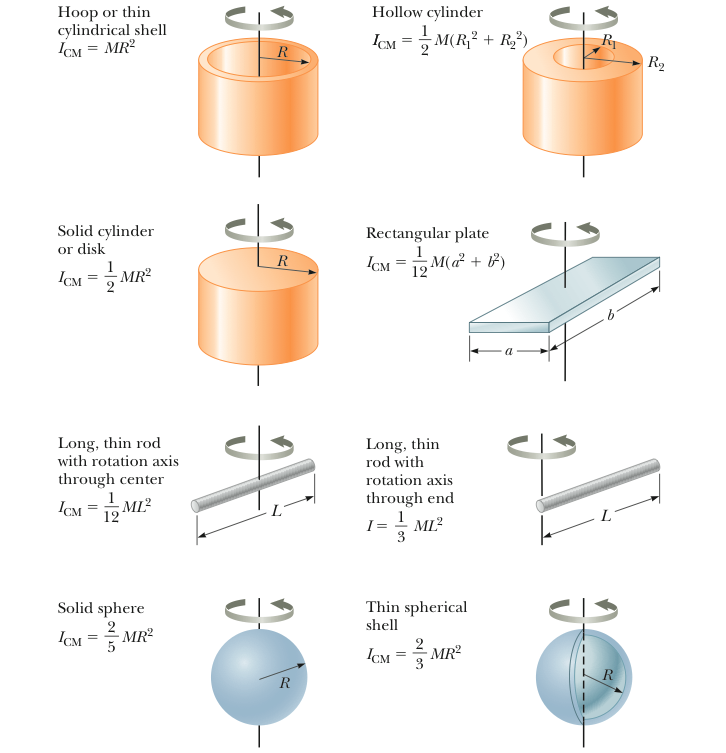
\includegraphics[height=0.5\textheight]{inertia.png}

\section{Newton's Second Law for Rotation}
\paragraph{Torque $\tau$}
$$\tau = rF_t = rF\sin \phi = F\ell$$

\paragraph{Work $W$}
$$\Delta W = F_tr\Delta \theta$$

\paragraph{Newton's Second Law for Rotation}
$$\sum \tau_\text{ext} = I\alpha$$

\paragraph{Power}
$$P = \frac{\Delta W}{\Delta t} = \frac{\tau\Delta\theta}{\Delta t} = \tau\omega$$

\section{Angular Momentum}
\paragraph{Angular Momentum $L$}
$$L = I\omega = r \times p$$

\paragraph{Conservation of Angular Momentum}
$L_\text{sys}$ is constant if the external torque on the system is 0.

\paragraph{Rolling}
When rigid objects roll, there are two types of basic rolling: ``with slipping'' and ``without slipping''. $$v_\text{cm} = R\omega$$

\end{document}
\end{document}